\documentclass[twoside,11pt]{article}

% Any additional packages needed should be included after jmlr2e.
% Note that jmlr2e.sty includes epsfig, amssymb, natbib and graphicx,
% and defines many common macros, such as 'proof' and 'example'.
%
% It also sets the bibliographystyle to plainnat; for more information on
% natbib citation styles, see the natbib documentation, a copy of which
% is archived at http://www.jmlr.org/format/natbib.pdf

% Available options for package jmlr2e are:
%
%   - abbrvbib : use abbrvnat for the bibliography style
%   - nohyperref : do not load the hyperref package
%   - preprint : remove JMLR specific information from the template,
%         useful for example for posting to preprint servers.
%
% Example of using the package with custom options:
%
% \usepackage[abbrvbib, preprint]{jmlr2e}
\usepackage[square,numbers]{natbib}
\bibliographystyle{abbrvnat}

\usepackage{jmlr2e}
\usepackage{graphicx}
\usepackage[ margin=1in]{geometry}
\usepackage{hyperref}
\hypersetup{colorlinks,linkcolor={purple},citecolor={blue},urlcolor={red}}  

% Definitions of handy macros can go here

\newcommand{\dataset}{{\cal D}}
\newcommand{\fracpartial}[2]{\frac{\partial #1}{\partial  #2}}

% Heading arguments are {volume}{year}{pages}{date submitted}{date published}{paper id}{author-full-names}

%\jmlrheading{1}{2000}{1-48}{4/00}{10/00}{meila00a}{Marina Meil\u{a} and Michael I. Jordan}

% Short headings should be running head and authors last names
\usepackage{fancyhdr}%
\usepackage{lipsum}% Just for this example


\fancyhf{}% Clear all headers/footers
\fancyfoot[L]{}\fancyfoot[C]{Belhal Karimi, Research Statement}\fancyfoot[R]{}
\renewcommand{\headrulewidth}{0pt}
\pagestyle{fancy}
\rfoot{\thepage}
%\thispagestyle{plain}

%\ShortHeadings{Belhal Karimi, Research Statement}{Belhal Karimi, Research Statement}
\firstpageno{1}
\newlength\tindent
\setlength{\tindent}{\parindent}
\setlength{\parindent}{0pt}
\renewcommand{\indent}{\hspace*{\tindent}}
\renewcommand{\refname}{}
\usepackage[dvipsnames]{xcolor}
\definecolor{mygray}{gray}{0.3}


\begin{document}

%\title{Research Statement}
%
%\author{\name Belhal Karimi \email belhal.karimi@gmail.com \\
%       \addr Cognitive Computing Lab\
%       Baidu Research\\
%       Seattle, WA 98195-4322, USA}
%
%
%
%\maketitle
%
%\begin{abstract}%   <- trailing '%' for backward compatibility of .sty file
%...\end{abstract}
%
%\begin{keywords}
%...
%\end{keywords}
%
%\section{Introduction}


\textbf{\scalebox{2}{Research Statement}}  \hfill \textbf{\scalebox{1.5}{Belhal Karimi}} 

 \hfill \scalebox{1}{\textcolor{mygray}{\textsc{Baidu Research}}}

\hfill

Throughout my research, I focus on developing \emph{training}, also known as \emph{optimization}, methods for large-scale datasets.
There are several specificities to my work.

The broad panel of my work has application on various problems, datasets and domains.
To name a few, such learning task as stated above is crucial while fitting complex nonlinear models (mixed models, deep neural networks, mixture models) on tabular, image, textual data to tackle problems encountered in computer vision, drug development or natural language processing.



\lipsum[35]

\begin{figure}[h]
\centering
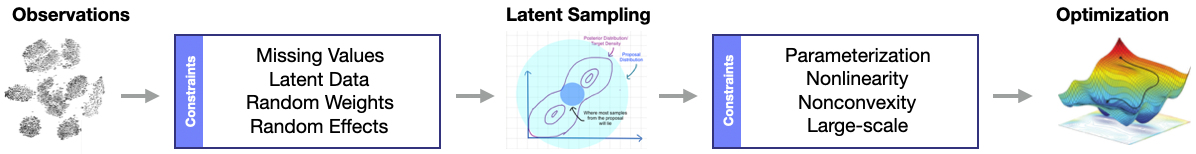
\includegraphics[width=\textwidth]{fig2}
%\caption{fhzuz}
\end{figure}
     
\lipsum[35]
\lipsum[35]


\vspace{0.2in}


% ---------------------------------------------------Deep Learning: Training and Generalization-----------------------------------------------------------------------------------------
\textbf{\scalebox{1.6}{(a) Deep Learning: Training and Generalization}}
\vspace{0.2in}

\lipsum[35]
\lipsum[5]
\vspace{0.15in}
\textbf{Training Acceleration} 
\vspace{0.08in}

\lipsum[35]


\vspace{0.15in}
\textbf{Decentralized Training} 
\vspace{0.08in}

\lipsum[35]

\vspace{0.15in}
\textbf{Towards Better Generalizaiton} 
\vspace{0.08in}

\lipsum[35]

\clearpage


% ---------------------------------------------------When Sampling meets Optimization-----------------------------------------------------------------------------------------

\textbf{\scalebox{1.6}{(b) When Sampling meets Optimization}}
\vspace{0.2in}

\lipsum[35]

\vspace{0.15in}
\textbf{Hierarchical Latent Structure Based Models} 
\vspace{0.08in}

\lipsum[35]


\vspace{0.15in}
\textbf{Two-level Stochastic Optimization Methods} 
\vspace{0.08in}

\lipsum[35]

\vspace{0.15in}
\textbf{MCMC Based Optimization} 
\vspace{0.08in}

\lipsum[35]

\newpage


% ---------------------------------------------------Future Research Directions-----------------------------------------------------------------------------------------
\textbf{\scalebox{1.6}{Future Research Directions}} 
\vspace{0.2in}

\lipsum[35]

\vspace{0.08in}
\paragraph{Energy Based Models.} \lipsum[35]

\vspace{0.08in}
\paragraph{Federated Learning.} \lipsum[35]

\vspace{0.08in}
\paragraph{Bayesian Deep Learning.} \lipsum[35]

\vspace{0.08in}
\paragraph{Stochastic Optimization for DNNs.} \lipsum[35]


\newpage


% ---------------------------------------------------References-----------------------------------------------------------------------------------------

\textbf{\scalebox{1.6}{References}}
\vspace{-0.3in}
\nocite{*}
\bibliography{references}

\end{document}
